\documentclass[a4paper,11pt]{article}

\usepackage{pgf}
\usepackage{tikz}
\usetikzlibrary{automata,positioning, arrows}

\usepackage[utf8]{inputenc}
\usepackage[spanish,es-noshorthands]{babel}




\usepackage[T1]{fontenc}
\usepackage{lmodern}
\usepackage{float}
 
\usepackage{parskip}
\usepackage{graphicx}
\usepackage{xcolor}
\usepackage{amsmath}

\begin{document}
    \begin{titlepage}
        \vspace*{1cm}
        % Logo
        
\includegraphics[width=\textwidth]{images/logos-fcefyn-y-unc.png} \\
        \\
        {\fontsize{28}{34}\selectfont\bfseries Programación Concurrente} \\
        {\fontsize{28}{34}\selectfont\bfseries Trabajo Práctico III}
        \hfill
        
        % Línea gris
        {\color{gray}\hrule}
        \Large{\itshape Redes de Petri para simular un procesador de 2 núcleos}
        
        \vfill
   Docentes: 
    \begin{itemize}
        \item Dr. Ing. Micolini Orlando
        \item Ing. Ventre, Luis
        \item Ing. Mauricio, Ludemann
    \end{itemize} 
        \vfill
        
        {\textbf{Benitez}, Darío Jeremías} \\
        {\textbf{Perez}, Bruno Santiago \hfill \today}
    \end{titlepage}


    \tableofcontents

    \pagebreak

    \section{Consigna}
    
    Se debe implementar un simulador de un procesador con dos núcleos. A partir de la red de
    Petri de la figura \ref{fig:procesador_mononucleo}, la cual representa a un procesador mono núcleo, se deberá extender la
    misma a una red que modele un procesador con dos núcleos. Además, se debe
    implementar una Política que resuelva los conflictos que se generan con las transiciones
    que alimentan los buffers de los núcleos (CPU\_Buffer).
    
    \begin{figure}[H]
        \centering
        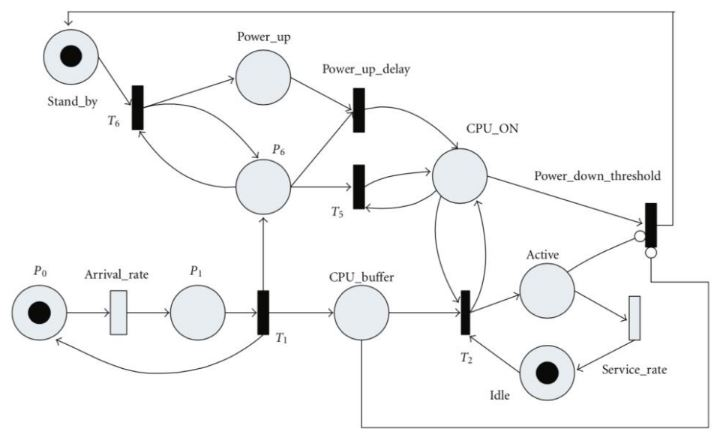
\includegraphics[width=1\textwidth]{images/enunciado_red_mononucleo.jpg}
        \caption{Red de petri para un procesador mononúcleo}
        \label{fig:procesador_mononucleo}
    \end{figure}
    
    \small{Nota: Las transiciones “Arrival\_rate” y “Service\_rate” son temporizadas y representan el
    tiempo de arribo de una tarea y el tiempo de servicio para concluir una tarea.}
    
    \section{Red de petri resultante}
    Para lograr un mejor entendimiento del problema se pasó la Red de Petri planteada en la consigna
    al software PIPE, se extendió la red para que consista de 
    2 procesadores y se renombraron las transiciones y plazas 
    para poder seguir mejor el estado de la red.
    
    La red resultante fue la siguiente:
    
    \begin{figure}[H]
        \centering
        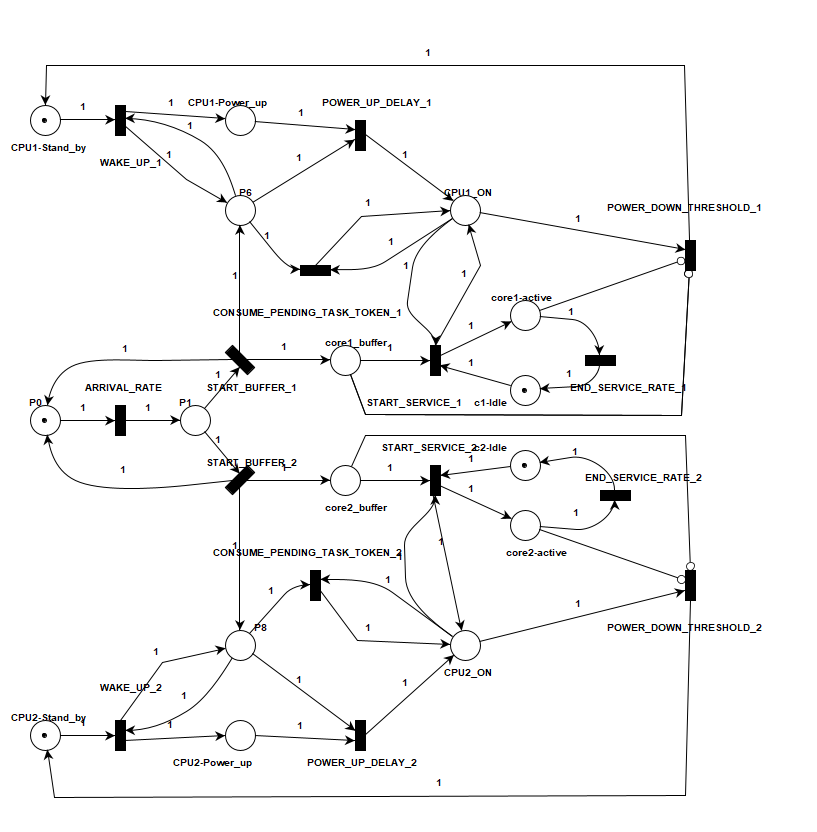
\includegraphics[width=1\textwidth]{images/red_final.png}
        \caption{Red de petri extendida de 2 núcleos}
        \label{fig:red_final}
    \end{figure}
    
    \section{Diseño}
    \subsection{Diagrama de clases}
    Para poder llevar a cabo la implementación de la red
    en JAVA se realizó un diagrama de clases para tener en claro
    las relaciones entre los objetos.
    \begin{figure}[H]
        \centering
        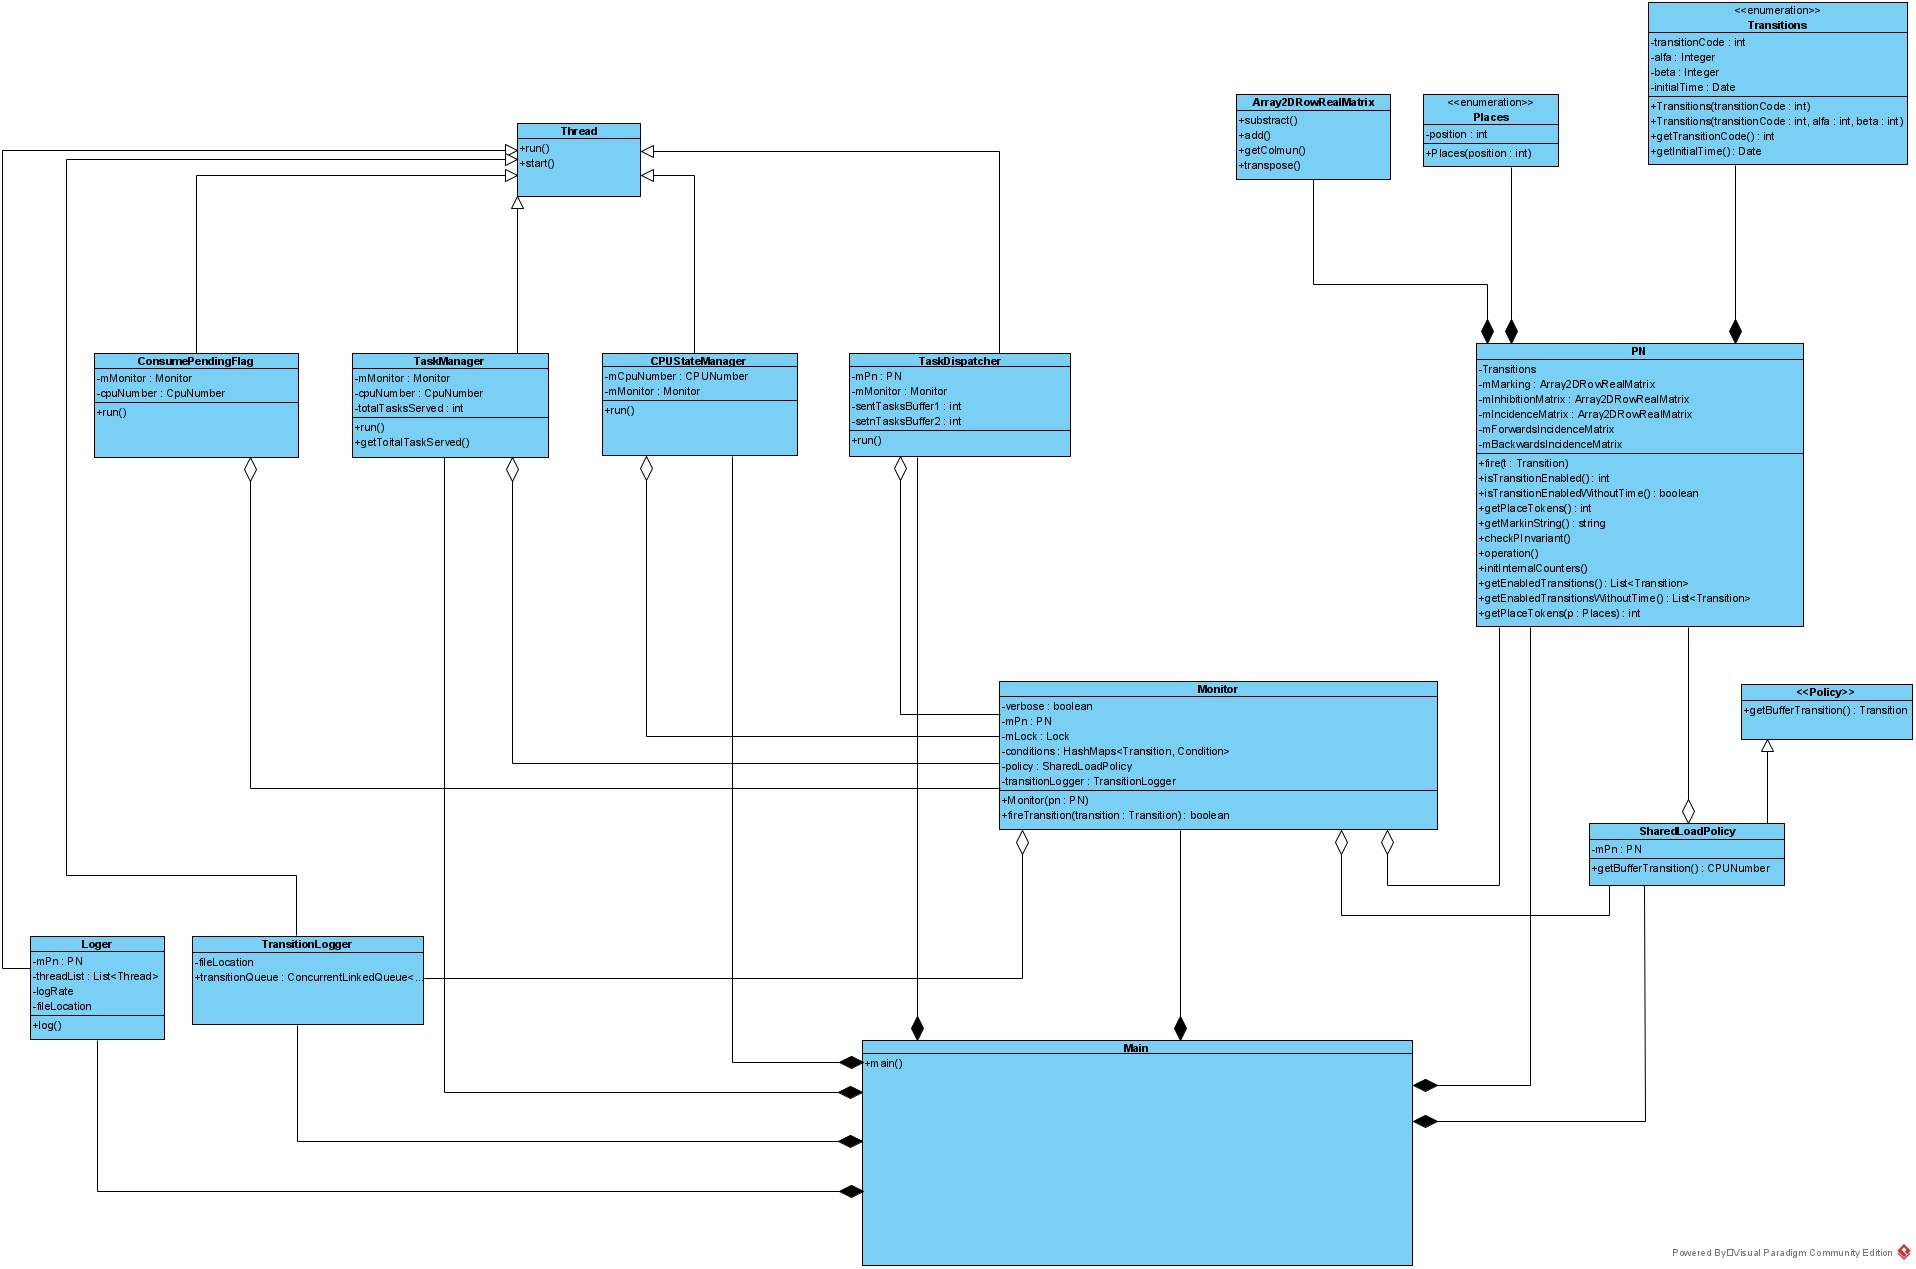
\includegraphics[width=1\textwidth]{images/diagrama_clases.jpg}
        \caption{Diagrama de clases del proyecto. Se puede ver en los adjuntos como \textit{diagrama\_clases.jpg}.}
        \label{fig:diag_clases}
    \end{figure}
    
    \subsection{PN (red de petri)}
    Esta clase contiene la funcionalidad la red de Petri.
    Tiene 2 elementos claves
    
    Tiene 3 clases fundamentales
    \begin{enumerate}
        \item 4 Matrices:
        \begin{itemize}
            \item mIncidenceMatrix
            \item mForwardsIncidenceMatrix
            \item mBackwardsIncidenceMatrix
            \item mInhibitionMatrix
            \item mMarking
        \end{itemize}
        \item Places: contiene las plazas de la RdP
        \item Transitions: enumeración que tiene información sobre las trancisiones, su relacion respecto a las matrices y su alfa y beta
    \end{enumerate}
    
    \subsection{Monitor}
    Es el mecanismo que nos permite acceder a la red de petri 
    de manera concurrente y efectuar disparos.
    
    Tiene una referencia a la clase Red de Petri para disparar transiciones mediante el método fire.
    Además tiene un método taskdispatch que despacha las tareas al CPU correspondiente
    de acuerdo a la política. Esto implica un acomplamiento indeseado entre el monitor y el
    problema en sí, pero como la política debía leer el estado de la red tuvimos que poner esa lógica
    en el monitor.
    
    \subsection{Hilos que manejan la RdP}
    Además hay 4 clases que conformarán 7 hilos:
    \begin{enumerate}
        \item ConsumePendingFlag (2 hilos para las 2 CPU)
        \item TaskManager (2 hilos para las 2 CPU)
        \item CPUStateManager (2 hilos para las 2 CPU)
        \item TaskDispatcher (1 solo hilo)
    \end{enumerate}
    \subsection{Loggers}
    Para el desarrollo del proyecto se necesitó de 2 loggers:
    \begin{enumerate}
        \item Logger: es el encargado de cada cierta frecuencia loguear el estado de los hilos, el marcado, y la carga en los buffers
        \item TransitionLogger: es el encargado de registar las transiciones disparadas y guardarlo en un archivo.
        Hace uso de la clase  ConcurrentLinkedQueue<String> para guardar las transiciones a medida que son disparadas y consumir esa cola a medida que se puede ir imprimiendo las transiciones en un archivo.
    \end{enumerate}
    \subsection{Policy}
    Se define una interfaz Policy que define un contrato en el cual se debe especificar qué transicion de buffer disparar.
    Tenemos una sola implementación que es la clase SharedLoadPolicy. Como el 
    nombre lo indica actúa como un balanceador de carga, es decir que va a intentar
    elegir la CPU que esté menos congestionada y en caso de que estén igualmente congestionadas elige la CPU más
    veloz.
    
    \section{Implementación}
    \subsection{Main}
    Contiene las referencias los hilos que disparan transiciones a través del monitor,
    al monitor en sí, a la RdP y a los Loggers.
    Se encarga de inicializar el sistema y de finalizarlo.
    
    \subsubsection{Hilos disparadores de transiciones}
    \begin{figure}[H]
        \centering
        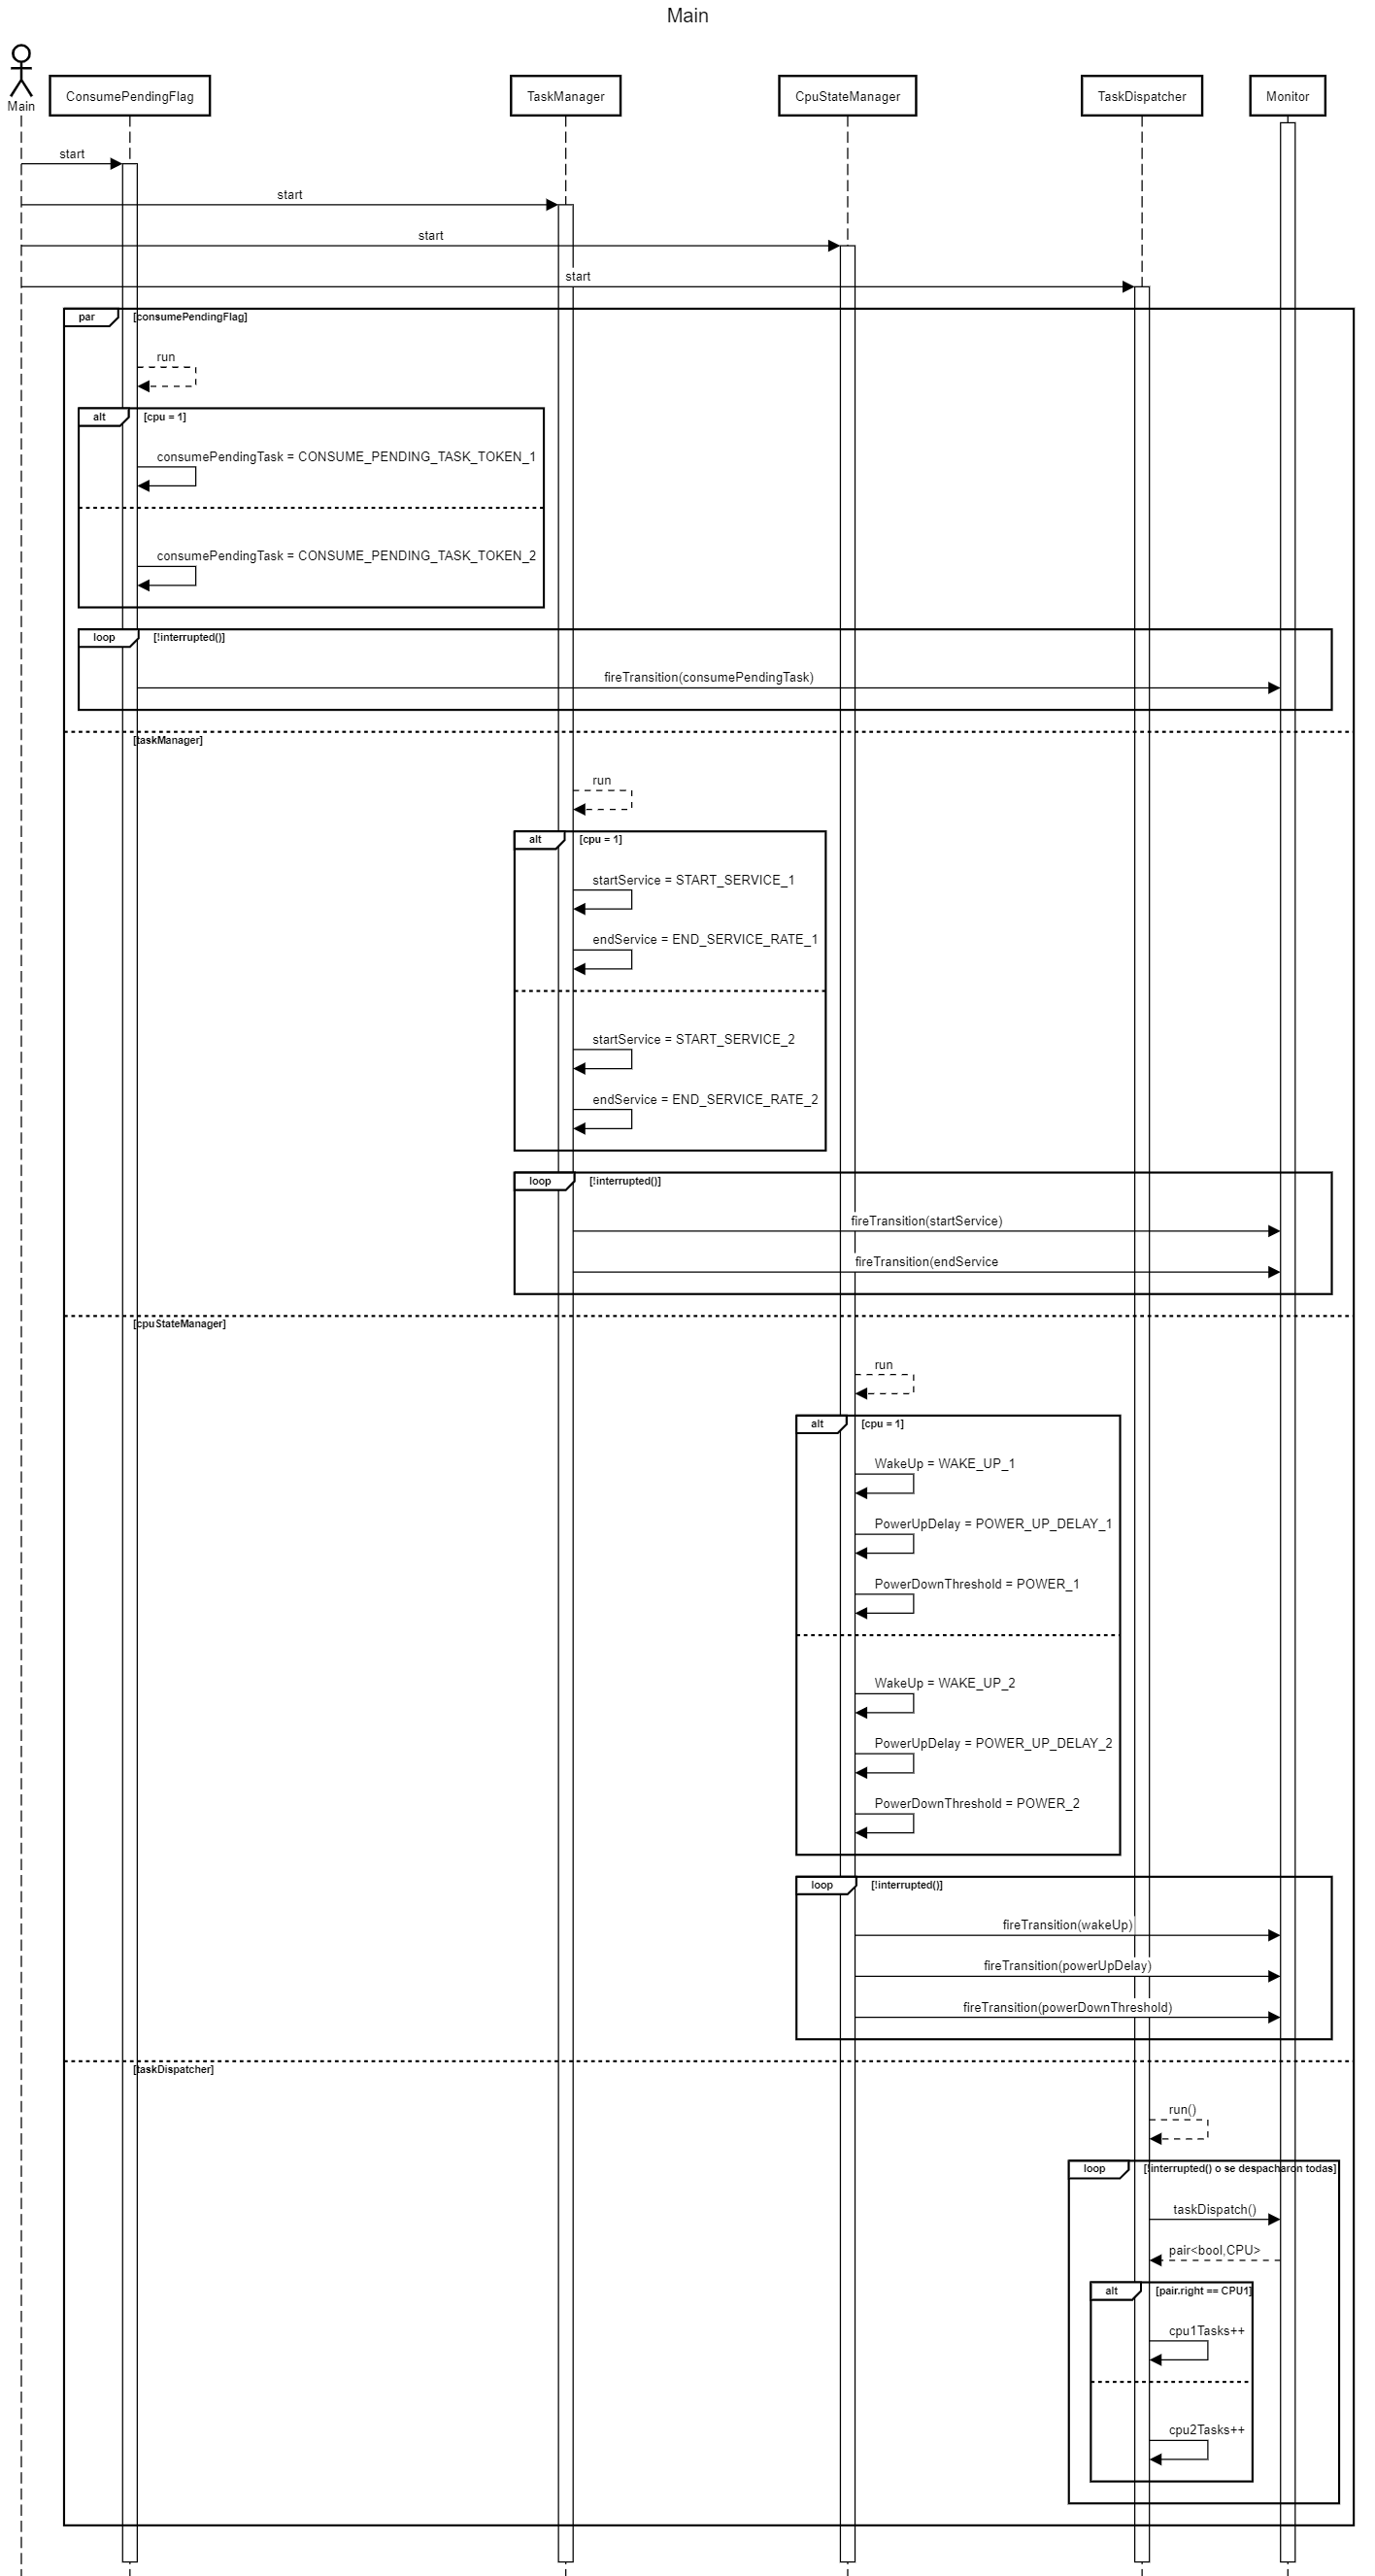
\includegraphics[width=0.8\textwidth]{sequence_diag/exports/Main.png}
        \caption{Diagrama de secuencia Main enfocandose en los disparos efectuados a traves del monitor}
        \label{fig:seq_Main}
    \end{figure}

    \subsection{PN}
    Para la implementación se comenzó con la red de Petri.
    Se explicarán los métodos más importantes.
    \subsubsection{IsTransitionEnabled(t)}
    Se encarga de decir si una transición t está habilitada sea o no temporizada.
    Respuestas:
    \begin{itemize}
        \item 1 si está habilitada sea o no temporizada
        \item 0 si no está habilitada o se pasó del tiempo beta
        \item -\{tiempo\} si no está habilitada pero en \{tiempo\} milisegundos se habilitará
    \end{itemize} 
    \begin{figure}[H]
        \centering
        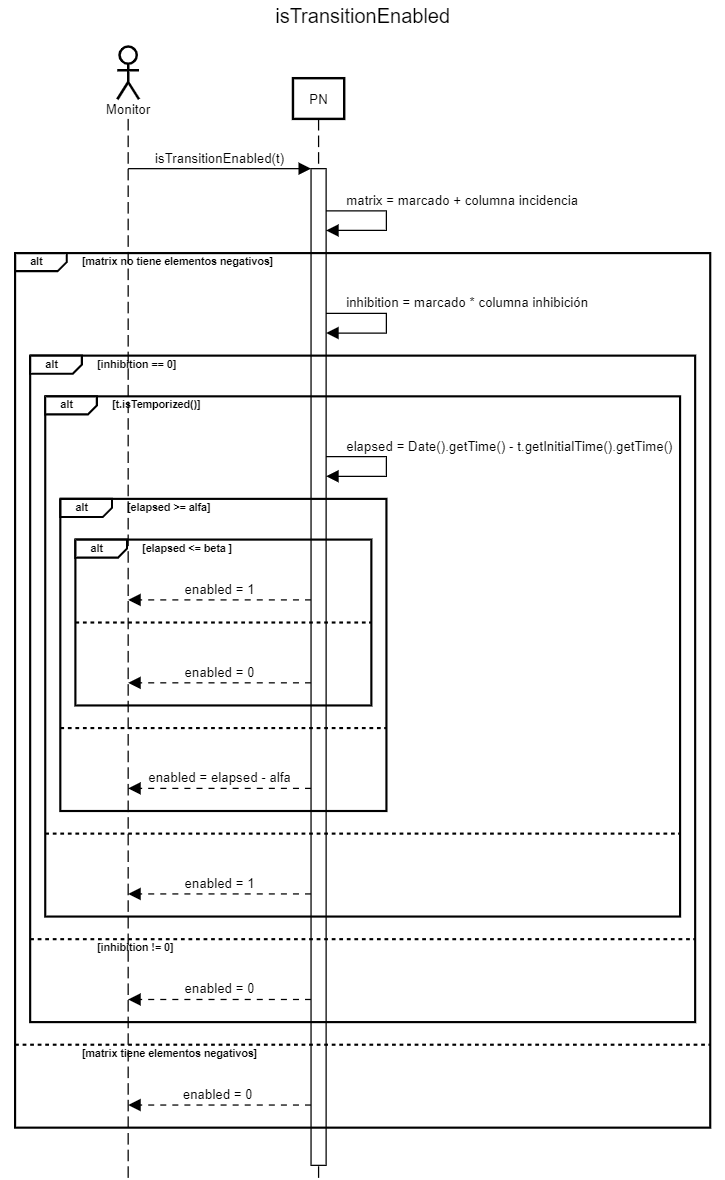
\includegraphics[width=0.8\textwidth]{sequence_diag/exports/IsTranstionEnabled.png}
        \caption{Diagrama de secuencia de IsTranstionEnabled}
        \label{fig:seq_IsTranstionEnabled}
    \end{figure}
    \subsection{Monitor}
    \subsubsection{Fire}
    Se encarga de disparar una transición.
    Devuelve True si se pudo ejectutar el disparo, False si no se pudo.
    \begin{figure}[H]
        \centering
        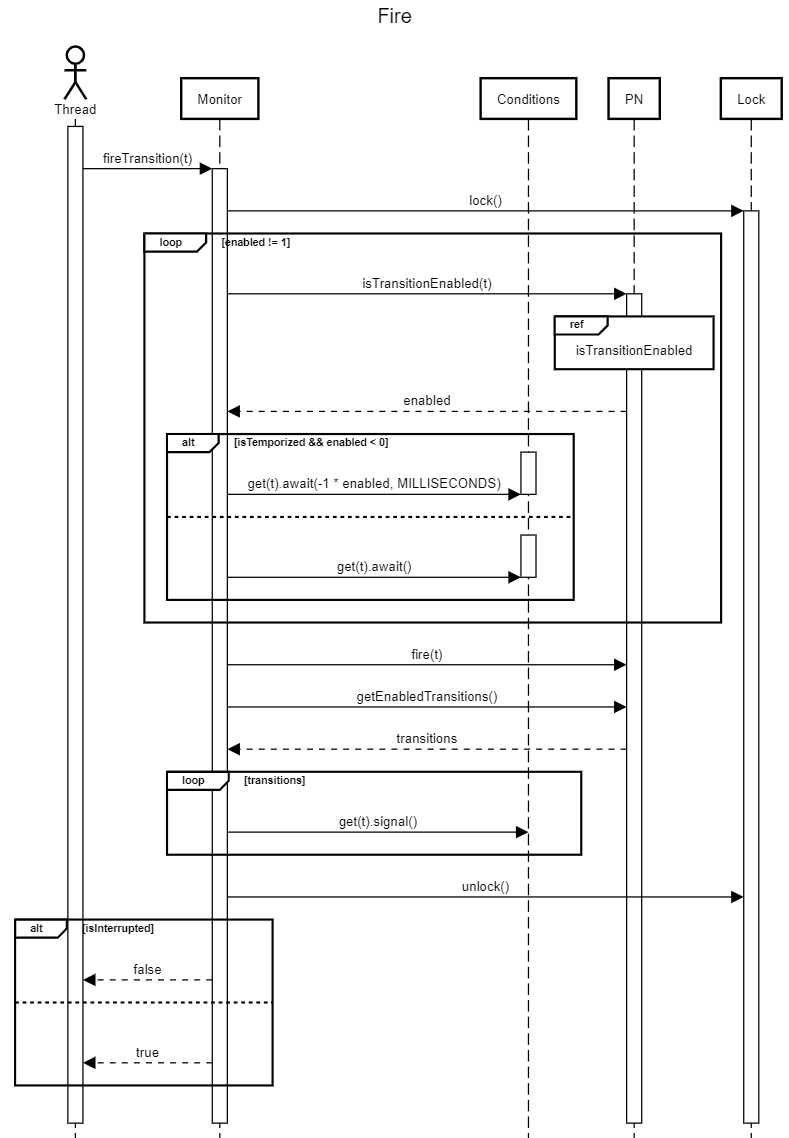
\includegraphics[width=0.8\textwidth]{sequence_diag/exports/Fire.png}
        \caption{Diagrama de secuencia de fire}
        \label{fig:seq_Fire}
    \end{figure}
    \subsubsection{TaskDispatch}
    Se utiliza para despachar una tarea. Utiliza al objeto política para 
    determinar hacia qué buffer despachar una tarea.
    \begin{figure}[H]
        \centering
        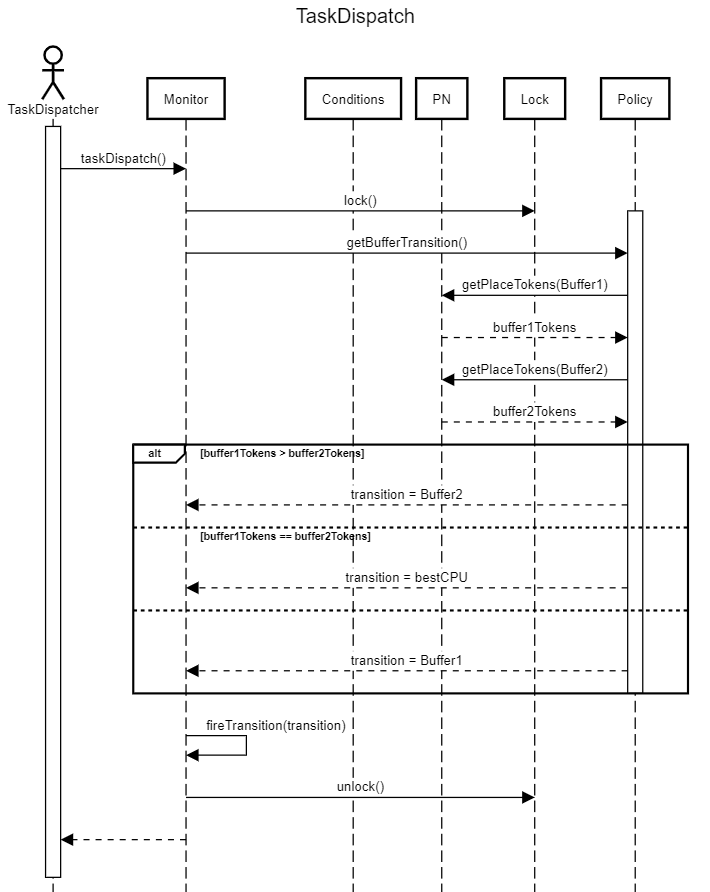
\includegraphics[width=0.8\textwidth]{sequence_diag/exports/TaskDispatch.png}
        \caption{Diagrama de secuencia de taskdispatch}
        \label{fig:seq_taskdispatch}
    \end{figure}

\end{document}  
